\label{cap:standDerTechnik}
Dieses Kapitel befasst sich mit dem aktuellen Stand der Technik. Dies
umfasst sowohl die gegenw{\"a}rtig eingesetzte Hardware, als auch bereits
entwickelte Protokolle zur interplanetaren Kommunikation.

\section{Weltraum-Technologien}
\textbf{Mars Rover Curiosity} 

Der Mars Rover \textit{Curiosity} (Abbildung \ref{fig:Curiosity}) verf{\"u}gt
{\"u}ber einen RAD750 Prozessor von BAE-Systems.
Dieser hat eine Taktfrequenz von bis zu 200 MHz und kann 266 MIPS
verarbeiten\footnote{Dieser Prozessor ist verglichem mit der Hardware, die im
Verlauf dieser Arbeit zum Test des entwickelten Protokolls eingesetzt wurde
sehr schwach.}. Desweiteren verf{\"u}gt \textit{Curiosity} {\"u}ber einen
Arbeitsspeicher von 256 MB und einen Flash-Speicher von 2 GB. Zus{\"a}tzlich hat \textit{Curiosity} einen EPROM von 256 KB. Alle Bauteile sind dabei besonders
strahlungsresistent und unempfindlich gegen{\"u}ber gro{\ss}en
Temperaturschwankungen. Das genutzte Betriebssystem ist VxWorks \cite{WR}.
Zur Kommunikation nutzt der Rover einerseits das X-Band (7 - 8 GHz), welches zur
{\"U}bertragung von Statusdaten und zum Empfang von Steuerdaten genutzt wird.
Des Weiteren verf{\"u}gt der Rover {\"u}ber ein Kommunikationssystem im UHF-Band
(0,4 GHz), welches f{\"u}r wissenschaftliche Daten mit hohem Datenvolumen
genutzt wird (bis zu 250 Mbit pro Tag, somit ca. 30 MB/Tag). Die Ausstattung an
wissenschaftlichen Instrumenten umfasst zehn Ger{\"a}te. Darunter z.B. zwei
Mastkameras welche je eine Aufl{\"o}sung von 1200 x 1200 Pixeln haben (1,44
Megapixel). Diese Kameras sind ebenfalls in der Lage 720p-Videos mit einer
Framerate von 10 Bildern pro Sekunde aufzunehmen. Hinzu kommen Spektrografen,
weitere Kameras, Sensoren etc., welche weitere Analysedaten beisteuern
\cite{web5}. Anhand der Vielzahl von Messinstrumenten, Kameras etc. wird
erkennbar, dass eine Menge unterschiedlicher Datentypen zu verwalten ist.
Desweiteren zeigt beispielsweise die Aufl{\"o}sung der Mastkameras, dass zudem
auch gro{\ss}e Datenmengen zu verwalten sind.

\begin{figure}[H]
\centering
\includegraphics[scale=.12]{Curiosity.png}
\caption[Mars Rover Curiosity]{Mars Rover Curiosity \cite{imgCuriosity}}
\label{fig:Curiosity}
\end{figure}

\textbf{Deep Space Network}

Das Deep Space Network bezeichnet ein Netz von Parabolantennen, welche zur
Kommunikation mit Raumsonden, Satelliten sowie zu radio-
und radarastronomischen Zwecken dienen. F{\"u}r die NASA werden derzeit die
folgenden drei gro{\ss}en Stationen betrieben:

\begin{compactenum}[a)]
\item \textit{Goldstone Deep Space Communication Complex, Kalifornien, USA
(Abbildung} \ref{fig:Goldstone}\textit{)}
\item \textit{Madrid Deep Space Communication Complex, Madrid, Spanien}
\item \textit{Canberra Deep Space Communication Complex, Canberra, Australien}
\end{compactenum}

Das Deep Space Network wird auch f{\"u}r die Kommunikation zwischen dem Mars
Rover \textit{Curiosity} und der Erde genutzt. Die Anlagen liegen an exponierter Position
(zumeist h{\"u}geliges schalenf{\"o}rmiges Gel{\"a}nde). Dies soll den
Einfluss von St{\"o}rungen z.B. durch Radiofrequenzen reduzieren. Die Stationen
befinden sich je in einem Abstand von einem drittel Erd{\"a}quator, um eine
fortw{\"a}hrende Kommunikation mit Raumfahrzeugen trotz Erdrotation zu
erm{\"o}glichen \cite{web6}.

\begin{figure}[H]
\centering
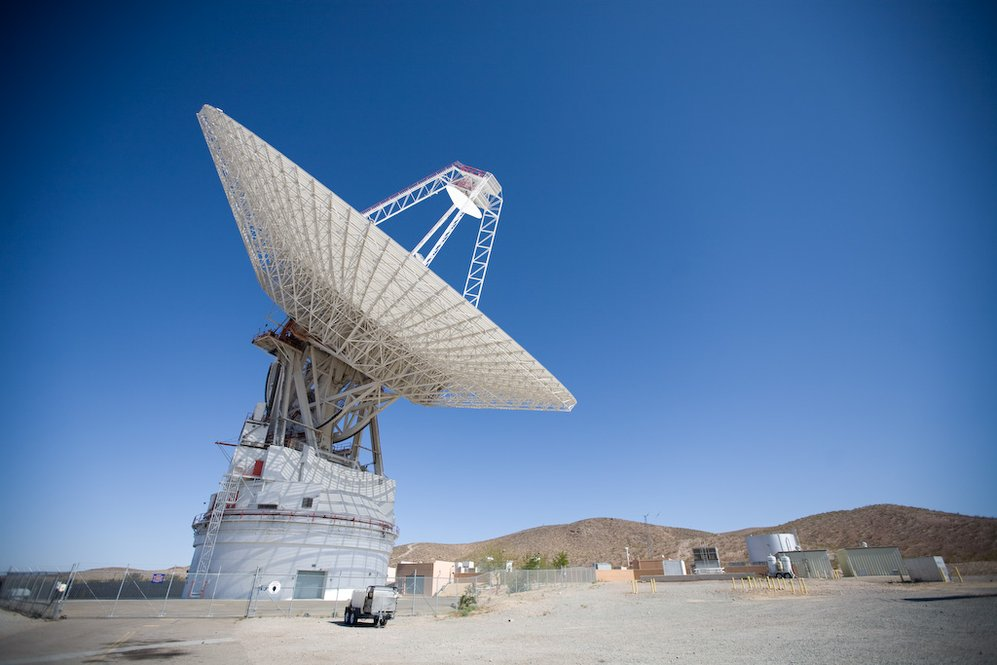
\includegraphics[scale=.3]{Goldstone.jpg}
\caption[Antenne der NASA Deep Space Network Einrichtung in Goldstone, Kalifornien, USA]
{Antenne der NASA Deep Space Network Einrichtung in Goldstone, Kalifornien, USA \cite{imgGoldstone}}
\label{fig:Goldstone}
\end{figure}

\section{Definitionen}

\textbf{Interplanetary Internet}

Das \gls{IPN} bezeichnet die Erweiterung des Internets
auf einen au{\ss}erirdischen Bereich. Die damit verbundenen {\"A}nderungen im
Vergleich zum irdischen Internet umfassen z.B. einen gesonderten Umgang mit
Latenzen, da diese beim \gls{IPN} im Minuten- bis Stundenbereich liegen. Die
Entwicklung von Protokollen f{\"u}r das \gls{IPN} obliegt dabei dem \gls{CCSDS}.

\textbf{Delay Tolerant Networking}

Das \gls{DTN} bezeichnet eine Protokollarchitektur f{\"u}r
Ende-zu-Ende Netzwerkverbindungen mit geringer Stabilit{\"a}t. Die Basis der
\gls{DTN} Netzwerkarchitektur stellt das von der NASA entwickelte \gls{IPN} dar. Ein wichtiger
Bestandteil dieser Netzwerke ist der Umgang mit gro{\ss}en Latenzen. Zudem
m{\"u}ssen die an der Kommunikation beteiligten Knoten (Teilnehmer)
Daten solange zwischenspeichern, bis der Empf{\"a}nger den Erhalt quittiert hat
(store-and-forward) \cite{web3}.

\section{Protokolle}

\textbf{Bundle-Protokoll}

Die in den RFCs 4838 und 5050 festgelegten Anforderungen f{\"u}r \gls{DTN} sind
weitgehend unter der Bezeichnung Bundle-Protokoll bekannt. In diesem werden
Folgen von Datenbl{\"o}cken als B{\"u}ndel zusammengefasst. Jedes B{\"u}ndel enth{\"a}lt
dabei ausreichende semantische Informationen, um eine etwaige Applikation
fortzusetzen. Exemplarisch sei hier ein Webbrowser angef{\"u}hrt, welcher ein
Bundle-Paket erh{\"a}lt und dadurch eine komplette Webseite anzeigt. Auch hier
erfolgt die {\"U}bertragung per \textit{store-and-forward}. Die eingesetzten
Transportprotokolle k{\"o}nnen dabei variieren (\gls{IP} basierend o.a.). Das
Bundle-Protokoll z{\"a}hlt zu den Overlay-Netzwerken, welche
auf einer bereits bestehenden Netzwerkstruktur aufsetzen \cite{web1}.

\textbf{Licklider Transmission Protocol}

Das \gls{LTP} kann direkt auf dem Data Link Layer
aufsetzen oder aber auch unter \gls{UDP} laufen (siehe Abb. \ref{fig:LTP}). Das \gls{LTP}
wird zudem als Standard \textit{convergence layer protocol} (Zusammenfassung von
Transport- und Network-Layer) f{\"u}r das Bundle Protokoll genutzt. Das \gls{LTP}
wurde zur sicheren {\"U}bertragung von Daten zwischen einem Sender und einem
Empf{\"a}nger (Punkt-zu-Punkt) unter \gls{DTN} Bedingungen entwickelt. Das \gls{LTP}
entscheidet dabei zwischen wichtigen (red data) und unwichtigen Daten (green
data) und gew{\"a}hrleistet somit eine effiziente {\"U}bermittlung. Eine
{\"U}bertragung beginnt, sobald ein Link zwischen Sender und Empf{\"a}nger
besteht. Die zu sendenden Datenbl{\"o}cke werden beim \gls{LTP} in Segmente geteilt.
Handelt es sich um wichtige Daten, werden w{\"a}hrend des Sendevorgangs
innerhalb der im \gls{LTP} verwendeten Segmente spezielle Flags gesetzt.
Diese einfach als Checkpoints bezeichneten Signale erfordern eine Quittierung
durch den Empf{\"a}nger, um so bei einem eventuellen Verbindungsabbruch ein
erneutes Senden des jeweiligen Datenpakets auszul{\"o}sen. Die Daten werden
solange beim Sender im Speicher (RAM oder lokaler Festspeicher z.B. Flash)
vorgehalten, bis der zugeh{\"o}rige Checkpoint quittiert wurde. Wenn ein Checkpoint nicht quittiert wird, kann durch
einen ablaufenden Timer auf der Seite des Senders ein erneutes Senden
durchgeführt werden. Sowohl das Senden als auch Empfangen eines Blocks kann per
Signal abgebrochen werden. Zudem ist die Gr{\"o}{\ss}e der Segmente einstellbar,
um diese an den jeweiligen Zweck anzupassen. Handelt es sich bei den zu sendenden
Daten um Daten mit geringerer Relevanz, so ist keine Best{\"a}tigung durch den
Empf{\"a}nger notwendig.
Diese Daten werden direkt nach dem Versenden gel{\"o}scht \cite{web4}.

\begin{figure}[H]
\centering
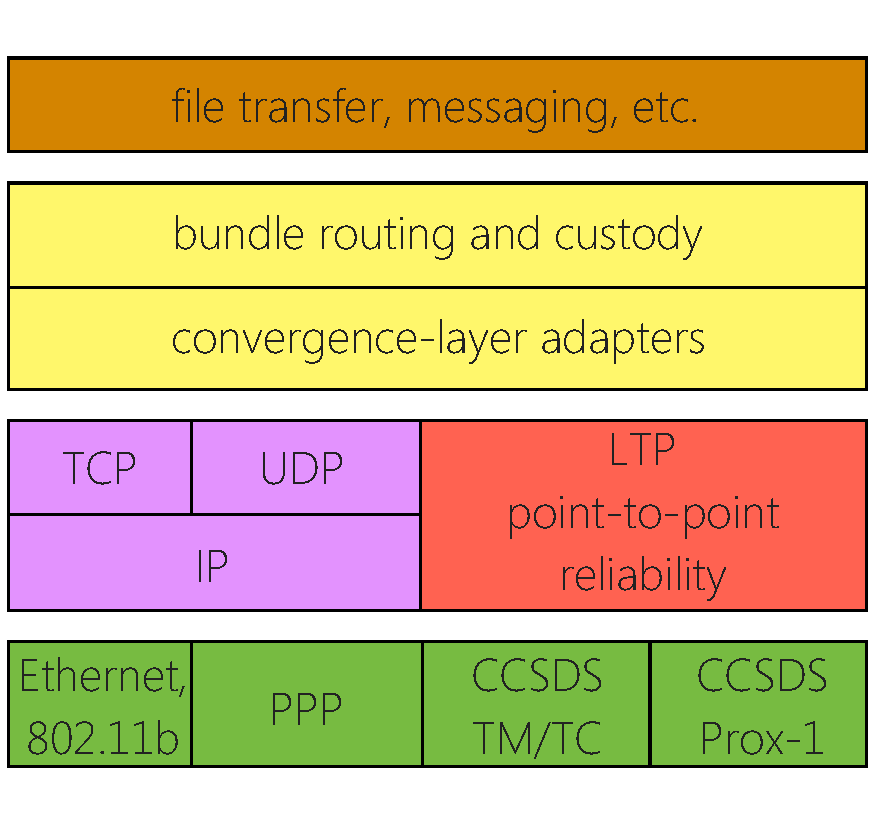
\includegraphics[scale=.4]{LTP.pdf}
\caption{Einordnung des LTP in das Kommunikationsmodell nach \cite{Burleigh}}
\label{fig:LTP}
\end{figure}

\textbf{Proximity-1}

Das \textit{Proximity-1 Space Link Protocol} ist das typischerweise genutzte
Data Link Layer/Physical Layer Protokoll in einem \gls{DTN} Stack. Damit komplettiert
dies zusammen mit dem Bundle Protokoll und dem \gls{LTP} die notwendigen
Protokollschichten eines \gls{DTN} Stack in einer interplanetaren Kommunikation.

\textbf{Stack einer interplanetaren Kommunikation}

Das \gls{DTN} Bundle Protokoll agiert als ein Overlay auf dem Transport Layer. Die
Abbildung \ref{fig:PSSBN} zeigt den Einsatz des Bundle Protokolls in einem
interplanetaren Kommunikationsansatz.
Dabei repr{\"a}sentiert der linke Teil des Stacks das Landefahrzeug auf der
Marsoberfl{\"a}che, welches das \gls{CFDP} {\"u}ber das Bundle Protokoll in
Verbindung mit dem \gls{LTP} nutzt.
Das Landefahrzeug wird schlie{\ss}lich {\"u}ber das Proximity-1 Space Link
Protokoll mit dem Orbiter (zweiter Stack von links) verbunden. Der dritte Stack
von links repr{\"a}sentiert z.B. eine \gls{DSN} Bodenstation. Der
Orbiter kommuniziert mit der \gls{DSN} Bodenstation {\"u}ber einen
\textit{deep-space-link} via Bundle Protokoll unter Nutzung des \gls{LTP}. Das
\gls{LTP} gew{\"a}hrleistet dabei eine verl{\"a}ssliche Verbindung. Der Stack
auf der rechten {\"a}u{\ss}eren Seite symbolisiert eine Missionskontrollstation,
welche mit der \gls{DSN} Bodenstation {\"u}ber einen klassische
\gls{TCP}/\gls{IP} Stack kommuniziert. Das Bundle Protokoll sichert dabei eine
Ende-zu-Ende Kommunikation \cite{DTNBundle}.

\begin{figure}[H]
\centering
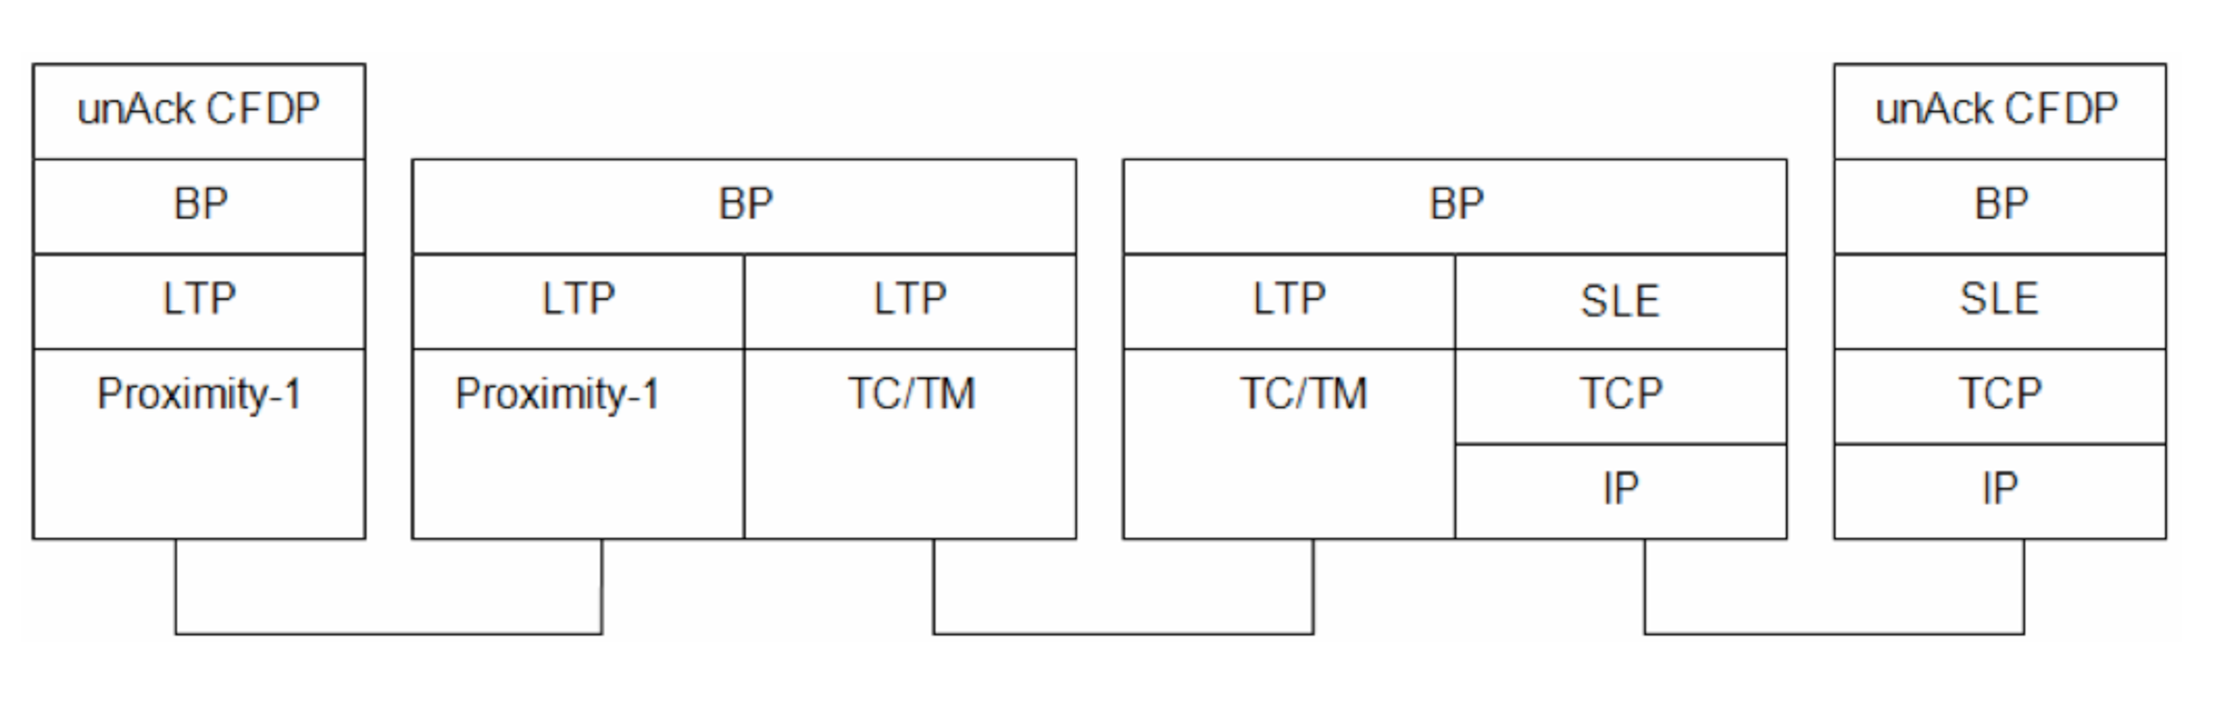
\includegraphics[scale=.35]{PSSBN.pdf}
\caption[Protokoll-Stack eines interplanetaren Netzwerks]
{Protokoll-Stack eines interplanetaren Netzwerks \cite{DTNBundle}}
\label{fig:PSSBN}
\end{figure}

\textbf{\gls{QoS} vs. \gls{QoI}}

Die G{\"u}te eines Kommunikationsdienstes wird in irdischen Netzwerken
{\"u}blicherweise als Quality of Service (QoS) bezeichnet. Hierbei gibt es eine
Auswahl von Qualit{\"a}tsmerkmalen, mit Hilfe derer die Qualit{\"a}t eines
Service bewertet werden kann. Im Beispiel eines IP-Netzwerks w{\"a}ren dies
Parameter wie Jitter \footnote{zeitl. Schwankung (Taktzittern) in der
{\"U}bertragung von Digitalsignalen}, Latenzzeit, die Paketverlustrate sowie der Datendurchsatz.
Das QoS-Modell ist zwar theoretisch auch auf eine interplanetare Kommunikation
anwendbar (z.B. DTN/IPN), jedoch gleicht dieses aufgrund der hohen Latenzzeiten
in der {\"U}bertragung eher einer postalischen Kommunikation. Aus diesem Grund
wurde mit dem QoI (Quality of Interaction) ein speziell f{\"u}r diesen
Anwendungsfall konzipiertes Verfahren entwickelt \cite{Daher2}. Dabei
werden, neben klassischen QoS-Merkmalen, welche ebenfalls genutzt werden
k{\"o}nnen, neue Verbindungsmerkmale betrachetet. Diese sind z.B. die
Dauer der Verbindung, {\"u}bertragene Daten pro Verbindung und andere Merkmale. 

\textbf{Ontologien}

Ontologien sind Sammlungen aus Inferenz- und Integrit{\"a}tsregeln, um
Schlussfolgerungen auf komplexe Probleme zu beziehen. Ontologien werden zum
Austausch von Wissen in digitaler Form genutzt.

Bestandteile einer Ontologie:

 \begin{compactenum}[I]
     \item \textit{Begriffe}
     \item \textit{Typen}
     \item \textit{Instanzen}
     \item \textit{Relationen}
     \item \textit{Vererbung}
     \item \textit{Axiome}
   \end{compactenum}
\newpage   
\textbf{Vergleich der aktuellen Technologien mit CRODT}

Das CRODT-Framework stellt eine umfangreiche Sammlung an Funktionalit{\"a}ten
zur Verf{\"u}gung. Diese {\"a}hneln in ihrem Einsatz zum Teil denen der
vorgestellten Protokolle (LTP/Bundle Protokoll). So unterscheidet das LTP
beispielsweise nach wichtigen und unwichtigen Daten (red/green data). Diese
Funktionalit{\"a}t gleicht in ihrer Intension der Relevanzevaluierung im
CRODT-Framework. Zudem sollen die Datenbl{\"o}cke aus den Messages, die durch
CROP verschickt werden, auf Seiten des Empf{\"a}ngers direkt lesbar sein. Diese
Funktionalit{\"a}t gleicht der Bundle-Strategie des Bundle Protokolls. Der
Einsatzgedanke der Ontologien innerhalb des CRODT-Frameworks hingegen,
unterscheidet sich deutlich von den anderen angef{\"u}hrten Protokollen. Hierbei
sollen wichtige Daten automatisch erkannt und bewertet werden. Zudem ist das
Contentsplitting und die Relevanzevaluierung innerhalb von CRODT wesentlich
differenzierter (Werte zwischen 0 und 100). Die eigentliche {\"U}bertragung
erfolgt beim CRODT-Framework bisher paketorientiert und ungesichert. Eine LTP
{\"a}hnliche Ende-zu-Ende Verbindung mit einer Empfangsquittierung w{\"a}re
jedoch auch denkbar.
